% Options for packages loaded elsewhere
\PassOptionsToPackage{unicode}{hyperref}
\PassOptionsToPackage{hyphens}{url}
%
\documentclass[
]{article}
\usepackage{lmodern}
\usepackage{amssymb,amsmath}
\usepackage{ifxetex,ifluatex}
\ifnum 0\ifxetex 1\fi\ifluatex 1\fi=0 % if pdftex
  \usepackage[T1]{fontenc}
  \usepackage[utf8]{inputenc}
  \usepackage{textcomp} % provide euro and other symbols
\else % if luatex or xetex
  \usepackage{unicode-math}
  \defaultfontfeatures{Scale=MatchLowercase}
  \defaultfontfeatures[\rmfamily]{Ligatures=TeX,Scale=1}
\fi
% Use upquote if available, for straight quotes in verbatim environments
\IfFileExists{upquote.sty}{\usepackage{upquote}}{}
\IfFileExists{microtype.sty}{% use microtype if available
  \usepackage[]{microtype}
  \UseMicrotypeSet[protrusion]{basicmath} % disable protrusion for tt fonts
}{}
\makeatletter
\@ifundefined{KOMAClassName}{% if non-KOMA class
  \IfFileExists{parskip.sty}{%
    \usepackage{parskip}
  }{% else
    \setlength{\parindent}{0pt}
    \setlength{\parskip}{6pt plus 2pt minus 1pt}}
}{% if KOMA class
  \KOMAoptions{parskip=half}}
\makeatother
\usepackage{xcolor}
\IfFileExists{xurl.sty}{\usepackage{xurl}}{} % add URL line breaks if available
\IfFileExists{bookmark.sty}{\usepackage{bookmark}}{\usepackage{hyperref}}
\hypersetup{
  pdftitle={Supplementary Material for `Winter Cover Cropping Effects on Soil Water-Holding Capacity Vary by Site'},
  pdfauthor={Nichols et al.~2021},
  hidelinks,
  pdfcreator={LaTeX via pandoc}}
\urlstyle{same} % disable monospaced font for URLs
\usepackage[margin=1in]{geometry}
\usepackage{graphicx,grffile}
\makeatletter
\def\maxwidth{\ifdim\Gin@nat@width>\linewidth\linewidth\else\Gin@nat@width\fi}
\def\maxheight{\ifdim\Gin@nat@height>\textheight\textheight\else\Gin@nat@height\fi}
\makeatother
% Scale images if necessary, so that they will not overflow the page
% margins by default, and it is still possible to overwrite the defaults
% using explicit options in \includegraphics[width, height, ...]{}
\setkeys{Gin}{width=\maxwidth,height=\maxheight,keepaspectratio}
% Set default figure placement to htbp
\makeatletter
\def\fps@figure{htbp}
\makeatother
\setlength{\emergencystretch}{3em} % prevent overfull lines
\providecommand{\tightlist}{%
  \setlength{\itemsep}{0pt}\setlength{\parskip}{0pt}}
\setcounter{secnumdepth}{-\maxdimen} % remove section numbering
\usepackage{float}
\floatplacement{figure}{H}
\usepackage{booktabs}
\usepackage{longtable}
\usepackage{array}
\usepackage{multirow}
\usepackage{wrapfig}
\usepackage{float}
\usepackage{colortbl}
\usepackage{pdflscape}
\usepackage{tabu}
\usepackage{threeparttable}
\usepackage{threeparttablex}
\usepackage[normalem]{ulem}
\usepackage{makecell}

\title{Supplementary Material for `Winter Cover Cropping Effects on Soil
Water-Holding Capacity Vary by Site'}
\author{Nichols et al.~2021}
\date{6/15/2021}

\begin{document}
\maketitle

\hypertarget{supplemental-material-s1.-map-of-sites}{%
\section{Supplemental material S1. Map of
sites}\label{supplemental-material-s1.-map-of-sites}}

\begin{figure}
\centering
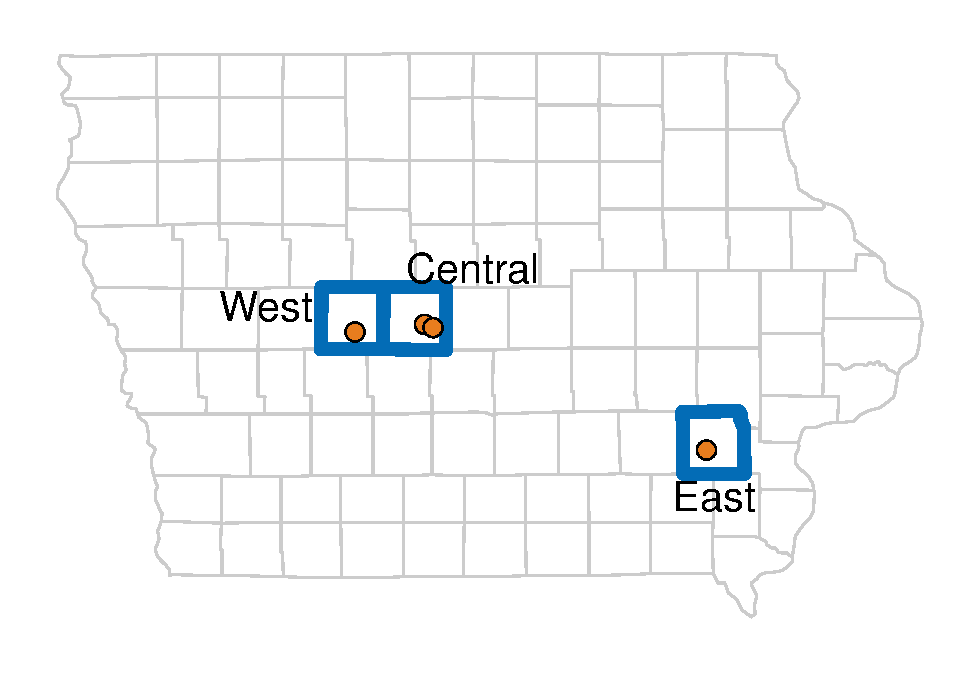
\includegraphics{rmd-supp-mat_files/figure-latex/sitemap-1.pdf}
\caption{Map of site locations in Iowa}
\end{figure}

\hypertarget{supplemental-material-s2.-general-site-management-summary}{%
\section{Supplemental material S2. General Site Management
Summary}\label{supplemental-material-s2.-general-site-management-summary}}

\begin{table}[H]

\caption{\label{tab:gentbl}General Site Description}
\centering
\begin{tabular}[t]{>{\centering\arraybackslash}p{5em}>{\centering\arraybackslash}p{5em}>{\centering\arraybackslash}p{5em}>{\centering\arraybackslash}p{3em}>{\centering\arraybackslash}p{3em}>{\centering\arraybackslash}p{3em}c}
\toprule
Site Description & General Location & Treatment Description & Year of Initiation & Crop Planted in 2019 & Number of Treatment Replicates & Sampled in 2019\\
\midrule
\cellcolor{gray!6}{} & \cellcolor{gray!6}{Boyd Farm, Boone, field 44} & \cellcolor{gray!6}{maize/soybean grain rotation, with and without rye cover crop} & \cellcolor{gray!6}{2009} & \cellcolor{gray!6}{maize} & \cellcolor{gray!6}{5} & \cellcolor{gray!6}{Y}\\

\multirow{-2}{*}{\centering\arraybackslash Central Grain} & Boyd Farm, Boone, field 42 & maize/soybean grain rotation, with and without rye cover crop & 2009 & soy & 5 & Y\\
\cmidrule{1-7}
\cellcolor{gray!6}{} & \cellcolor{gray!6}{Boyd Farm, Boone, field 44} & \cellcolor{gray!6}{maize silage/soybean grain rotation, with and without rye cover crop} & \cellcolor{gray!6}{2002} & \cellcolor{gray!6}{maize silage} & \cellcolor{gray!6}{5} & \cellcolor{gray!6}{Y}\\

\multirow{-2}{*}{\centering\arraybackslash Central Silage} & Boyd Farm, Boone, field 42 & maize silage/soybean grain rotation, with and without rye cover crop & 2002 & soy & 5 & N\\
\cmidrule{1-7}
\cellcolor{gray!6}{West} & \cellcolor{gray!6}{Jefferson, IA} & \cellcolor{gray!6}{maize/soybean grain rotation, with and without rye cover crop} & \cellcolor{gray!6}{2008} & \cellcolor{gray!6}{maize} & \cellcolor{gray!6}{4} & \cellcolor{gray!6}{Y}\\
\cmidrule{1-7}
East & Washington, IA & maize/soybean grain rotation, with and without rye cover crop & 2009 & soybeans & 4 & Y\\
\bottomrule
\end{tabular}
\end{table}

\newpage

\begin{table}[H]

\caption{\label{tab:herbtable}2018-2019 Herbicide Use}
\centering
\begin{tabular}[t]{>{\centering\arraybackslash}p{8em}>{\centering\arraybackslash}p{8em}>{\centering\arraybackslash}p{8em}>{\centering\arraybackslash}p{8em}}
\toprule
Site Description & Herbicides Used in 2018 Growing Season & Herbicdes Used in Fall 2018 & Herbicides Used in Spring 2019\\
\midrule
\cellcolor{gray!6}{Central Grain} & \cellcolor{gray!6}{glyphosate 1 week before soybean planting} & \cellcolor{gray!6}{none} & \cellcolor{gray!6}{glyphosate 1 week before maize planting; metalochlor, atrazine, and mesotrione at planting}\\
\multirow{-2}{8em}{\centering\arraybackslash Central Grain} & glyphosate 1 week before maize planting; metalochlor, atrazine, and mesotrione at planting & none & glyphosate 1 week before soybean planting\\
\cmidrule{1-4}
\cellcolor{gray!6}{Central Silage} & \cellcolor{gray!6}{glyphosate 1 week before soybean planting} & \cellcolor{gray!6}{none} & \cellcolor{gray!6}{glyphosate 1 week before maize planting; metalochlor, atrazine, and mesotrione at planting}\\
\multirow{-2}{8em}{\centering\arraybackslash Central Silage} & glyphosate 1 week before maize planting; metalochlor, atrazine, and mesotrione at planting & none & glyphosate 1 week before soybean planting\\
\cmidrule{1-4}
\cellcolor{gray!6}{West} & \cellcolor{gray!6}{glyphosate before planting; glyphosate and fluthiacet-methyl at planting} & \cellcolor{gray!6}{none} & \cellcolor{gray!6}{glyphosate before planting; glyphosate and fluthiacet-methyl at planting}\\
East & glyphosate and acetochlor  before planting (April 15), atrazine, acetochlor at planting (May 14); acetochlor and glyphosate after planting (June 15) & none & chlorimuron-ethyl, flumioxazin, pyroxasulfone, and glyphosate before planting, dicamba and acetochlor after planting\\
\bottomrule
\end{tabular}
\end{table}

\newpage

\begin{table}[H]

\caption{\label{tab:mgmttable}General Management}
\centering
\begin{tabular}[t]{c>{\centering\arraybackslash}p{7em}>{\centering\arraybackslash}p{5em}>{\centering\arraybackslash}p{5em}>{\centering\arraybackslash}p{5em}>{\centering\arraybackslash}p{5em}>{\centering\arraybackslash}p{5em}}
\toprule
Site Description & General Herbicide Regime & General Date of Cover Crop Termination & General Date of Crop Planting & Inorganic Fertilizer Used & Organic Fertilizer Used & Tillage Used\\
\midrule
\cellcolor{gray!6}{Central Grain} & \cellcolor{gray!6}{burndown, residual herbicide at maize planting} & \cellcolor{gray!6}{15-Apr} & \cellcolor{gray!6}{26-Apr} & \cellcolor{gray!6}{Y} & \cellcolor{gray!6}{NA} & \cellcolor{gray!6}{N}\\
\multirow{-2}{*}{\centering\arraybackslash Central Grain} & burndown, residual herbicide at maize planting & 25-Apr & 5-May & Y & NA & N\\
\cmidrule{1-7}
\cellcolor{gray!6}{Central Silage} & \cellcolor{gray!6}{burndown, residual herbicide at maize planting} & \cellcolor{gray!6}{15-Apr} & \cellcolor{gray!6}{26-Apr} & \cellcolor{gray!6}{Y} & \cellcolor{gray!6}{NA} & \cellcolor{gray!6}{N}\\
\multirow{-2}{*}{\centering\arraybackslash Central Silage} & burndown, residual herbicide at maize planting & 25-Apr & 5-May & Y & NA & N\\
\cmidrule{1-7}
\cellcolor{gray!6}{West} & \cellcolor{gray!6}{burndown, pre-emergent herbicide} & \cellcolor{gray!6}{1-May} & \cellcolor{gray!6}{10-May} & \cellcolor{gray!6}{Y} & \cellcolor{gray!6}{chicken or turkey manure} & \cellcolor{gray!6}{N}\\
East & burndown, residual herbicide at planting, another application on maize at \textasciitilde{}V6 & 1-May & 5-May & Y & liquid swine, \textasciitilde{}3000 gal/ac every other year to entire field & N\\
\bottomrule
\end{tabular}
\end{table}

\newpage

Cover crop biomass production over past 10 years of trials

\begin{table}[H]

\caption{\label{tab:ccbio}Historical cover crop biomass production (Mg/ha) by trial}
\centering
\begin{tabular}[t]{ccccccccccc}
\toprule
trial & 2010 & 2011 & 2012 & 2013 & 2014 & 2015 & 2016 & 2017 & 2019 & 2018\\
\midrule
\cellcolor{gray!6}{Central\_grain} & \cellcolor{gray!6}{0.86} & \cellcolor{gray!6}{0.28} & \cellcolor{gray!6}{1.37} & \cellcolor{gray!6}{0.25} & \cellcolor{gray!6}{0.47} & \cellcolor{gray!6}{0.61} & \cellcolor{gray!6}{2.22} & \cellcolor{gray!6}{2.76} & \cellcolor{gray!6}{1.29} & \cellcolor{gray!6}{NA}\\
Central\_silage & 1.59 & 1.72 & 3.32 & 1.26 & 0.91 & 1.76 & 4.23 & 2.21 & 2.05 & NA\\
\cmidrule{1-11}
\cellcolor{gray!6}{East\_grain} & \cellcolor{gray!6}{2.11} & \cellcolor{gray!6}{1.46} & \cellcolor{gray!6}{0.00} & \cellcolor{gray!6}{0.92} & \cellcolor{gray!6}{0.00} & \cellcolor{gray!6}{0.36} & \cellcolor{gray!6}{0.51} & \cellcolor{gray!6}{7.30} & \cellcolor{gray!6}{0.30} & \cellcolor{gray!6}{0.19}\\
West\_grain & 2.11 & 0.21 & 1.33 & 0.00 & 0.00 & 0.04 & 0.45 & 0.63 & 0.00 & 0.09\\
\bottomrule
\end{tabular}
\end{table}

\newpage

\hypertarget{supplemental-material-s3.-soil-texture-results}{%
\section{Supplemental material S3. Soil texture
results}\label{supplemental-material-s3.-soil-texture-results}}

\begin{figure}
\centering
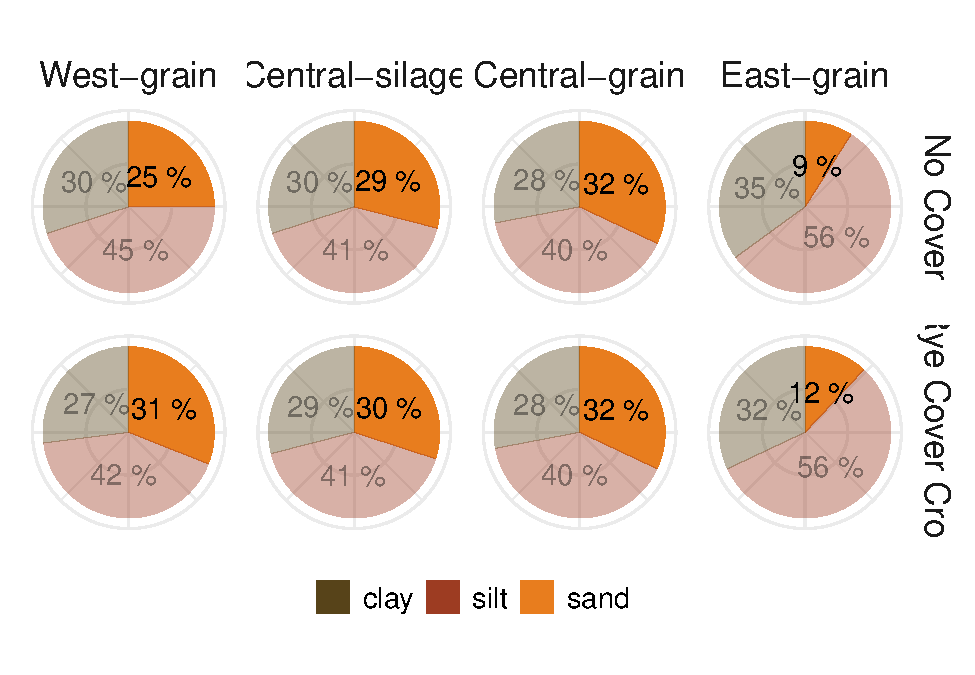
\includegraphics{rmd-supp-mat_files/figure-latex/texture-1.pdf}
\caption{Soil texture components varied by trial and cover crop
treatment, with the cover cropped plots having significantly more sand
bolded orange color, and significantly less clay at the West-grain and
East-grain trials both, commercial fields}
\end{figure}

Table with values:

\begin{table}[H]

\caption{\label{tab:texture2}Table of values}
\centering
\begin{tabular}[t]{ccccccc}
\toprule
site\_sys & cc\_trt & clay & sand & silt & tot & sig\_sand\_diff\\
\midrule
\cellcolor{gray!6}{} & \cellcolor{gray!6}{cc} & \cellcolor{gray!6}{0.28} & \cellcolor{gray!6}{0.32} & \cellcolor{gray!6}{0.40} & \cellcolor{gray!6}{1} & \cellcolor{gray!6}{}\\

\multirow{-2}{*}{\centering\arraybackslash Central-grain} & no & 0.28 & 0.32 & 0.40 & 1 & \\

\cellcolor{gray!6}{} & \cellcolor{gray!6}{cc} & \cellcolor{gray!6}{0.29} & \cellcolor{gray!6}{0.30} & \cellcolor{gray!6}{0.41} & \cellcolor{gray!6}{1} & \cellcolor{gray!6}{}\\

\multirow{-2}{*}{\centering\arraybackslash Central-silage} & no & 0.30 & 0.29 & 0.41 & 1 & \multirow{-4}{*}{\centering\arraybackslash No}\\
\cmidrule{1-7}
\cellcolor{gray!6}{} & \cellcolor{gray!6}{cc} & \cellcolor{gray!6}{0.32} & \cellcolor{gray!6}{0.12} & \cellcolor{gray!6}{0.56} & \cellcolor{gray!6}{1} & \cellcolor{gray!6}{}\\

\multirow{-2}{*}{\centering\arraybackslash East-grain} & no & 0.35 & 0.09 & 0.56 & 1 & \\

\cellcolor{gray!6}{} & \cellcolor{gray!6}{cc} & \cellcolor{gray!6}{0.27} & \cellcolor{gray!6}{0.31} & \cellcolor{gray!6}{0.42} & \cellcolor{gray!6}{1} & \cellcolor{gray!6}{}\\

\multirow{-2}{*}{\centering\arraybackslash West-grain} & no & 0.30 & 0.25 & 0.45 & 1 & \multirow{-4}{*}{\centering\arraybackslash Yes}\\
\bottomrule
\end{tabular}
\end{table}

\begin{table}[H]

\caption{\label{tab:texture2}Table of sand statistics}
\centering
\begin{tabular}[t]{cccccccc}
\toprule
site\_sys & respvar & cc & no & contrast & est\_diff & diff\_se & pval\\
\midrule
\cellcolor{gray!6}{Central\_grain} & \cellcolor{gray!6}{sand} & \cellcolor{gray!6}{32.486} & \cellcolor{gray!6}{31.600} & \cellcolor{gray!6}{cc - no} & \cellcolor{gray!6}{0.886} & \cellcolor{gray!6}{0.299} & \cellcolor{gray!6}{0.003}\\
Central\_silage & sand & 29.811 & 29.233 & cc - no & 0.578 & 0.335 & 0.085\\
\cellcolor{gray!6}{East\_grain} & \cellcolor{gray!6}{sand} & \cellcolor{gray!6}{12.715} & \cellcolor{gray!6}{9.837} & \cellcolor{gray!6}{cc - no} & \cellcolor{gray!6}{2.877} & \cellcolor{gray!6}{0.335} & \cellcolor{gray!6}{<0.001}\\
West\_grain & sand & 30.506 & 25.610 & cc - no & 4.896 & 0.335 & <0.001\\
\bottomrule
\end{tabular}
\end{table}

\hypertarget{supplemental-material-s4.-statistical-summaries}{%
\section{Supplemental material S4. Statistical
summaries}\label{supplemental-material-s4.-statistical-summaries}}

\begin{table}[H]

\caption{\label{tab:clay}Statistical analysis of cover crop effect on clay}
\centering
\begin{tabular}[t]{cccccccc}
\toprule
site\_sys & respvar & cc & no & contrast & est\_diff & diff\_se & diff\_pval\\
\midrule
\cellcolor{gray!6}{Central\_grain} & \cellcolor{gray!6}{clay} & \cellcolor{gray!6}{27.740} & \cellcolor{gray!6}{28.000} & \cellcolor{gray!6}{cc - no} & \cellcolor{gray!6}{-0.260} & \cellcolor{gray!6}{0.186} & \cellcolor{gray!6}{0.164}\\
Central\_silage & clay & 28.751 & 29.895 & cc - no & -1.144 & 0.208 & <0.001\\
\cellcolor{gray!6}{East\_grain} & \cellcolor{gray!6}{clay} & \cellcolor{gray!6}{31.730} & \cellcolor{gray!6}{34.606} & \cellcolor{gray!6}{cc - no} & \cellcolor{gray!6}{-2.876} & \cellcolor{gray!6}{0.208} & \cellcolor{gray!6}{<0.001}\\
West\_grain & clay & 27.349 & 29.511 & cc - no & -2.162 & 0.208 & <0.001\\
\bottomrule
\end{tabular}
\end{table}

\begin{table}[H]

\caption{\label{tab:clay}Statistical analysis of cover crop effect on sand}
\centering
\begin{tabular}[t]{cccccccc}
\toprule
site\_sys & respvar & cc & no & contrast & est\_diff & diff\_se & diff\_pval\\
\midrule
\cellcolor{gray!6}{Central\_grain} & \cellcolor{gray!6}{sand} & \cellcolor{gray!6}{32.486} & \cellcolor{gray!6}{31.600} & \cellcolor{gray!6}{cc - no} & \cellcolor{gray!6}{0.886} & \cellcolor{gray!6}{0.299} & \cellcolor{gray!6}{0.003}\\
Central\_silage & sand & 29.811 & 29.233 & cc - no & 0.578 & 0.335 & 0.085\\
\cellcolor{gray!6}{East\_grain} & \cellcolor{gray!6}{sand} & \cellcolor{gray!6}{12.715} & \cellcolor{gray!6}{9.837} & \cellcolor{gray!6}{cc - no} & \cellcolor{gray!6}{2.877} & \cellcolor{gray!6}{0.335} & \cellcolor{gray!6}{<0.001}\\
West\_grain & sand & 30.506 & 25.610 & cc - no & 4.896 & 0.335 & <0.001\\
\bottomrule
\end{tabular}
\end{table}

\begin{table}[H]

\caption{\label{tab:omstats}Statistical analysis of cover crop effect on organic matter, with and without sand covariate}
\centering
\begin{tabular}[t]{ccccccccc}
\toprule
cov & site\_sys & respvar & cc & no & contrast & est\_diff & diff\_se & diff\_pval\\
\midrule
\cellcolor{gray!6}{none} & \cellcolor{gray!6}{Central\_grain} & \cellcolor{gray!6}{om} & \cellcolor{gray!6}{2.360} & \cellcolor{gray!6}{2.480} & \cellcolor{gray!6}{cc - no} & \cellcolor{gray!6}{-0.120} & \cellcolor{gray!6}{0.051} & \cellcolor{gray!6}{0.02}\\
 & Central\_silage & om & 2.640 & 2.416 & cc - no & 0.224 & 0.057 & <0.001\\

\cellcolor{gray!6}{none} & \cellcolor{gray!6}{East\_grain} & \cellcolor{gray!6}{om} & \cellcolor{gray!6}{3.575} & \cellcolor{gray!6}{3.675} & \cellcolor{gray!6}{cc - no} & \cellcolor{gray!6}{-0.100} & \cellcolor{gray!6}{0.057} & \cellcolor{gray!6}{0.082}\\
\multirow{-4}{*}{\centering\arraybackslash none} & West\_grain & om & 2.750 & 2.975 & cc - no & -0.225 & 0.057 & <0.001\\
\cmidrule{1-9}
\cellcolor{gray!6}{sand} & \cellcolor{gray!6}{Central\_grain} & \cellcolor{gray!6}{om} & \cellcolor{gray!6}{3.034} & \cellcolor{gray!6}{3.066} & \cellcolor{gray!6}{cc - no} & \cellcolor{gray!6}{-0.032} & \cellcolor{gray!6}{0.082} & \cellcolor{gray!6}{0.696}\\
 & Central\_silage & om & 3.049 & 2.772 & cc - no & 0.278 & 0.088 & 0.002\\

\cellcolor{gray!6}{sand} & \cellcolor{gray!6}{East\_grain} & \cellcolor{gray!6}{om} & \cellcolor{gray!6}{2.290} & \cellcolor{gray!6}{2.105} & \cellcolor{gray!6}{cc - no} & \cellcolor{gray!6}{0.185} & \cellcolor{gray!6}{0.093} & \cellcolor{gray!6}{0.048}\\
\multirow{-4}{*}{\centering\arraybackslash sand} & West\_grain & om & 3.228 & 2.968 & cc - no & 0.260 & 0.096 & 0.007\\
\bottomrule
\end{tabular}
\end{table}

\begin{table}[H]

\caption{\label{tab:bulkden}Mean bulk density (g/cm3) by trial}
\centering
\begin{tabular}[t]{cccccc}
\toprule
site\_name & sys\_trt & crop\_trt & cc\_trt & bulkden\_mean & bulkden\_sd\\
\midrule
\cellcolor{gray!6}{Central} & \cellcolor{gray!6}{grain} & \cellcolor{gray!6}{soy} & \cellcolor{gray!6}{cc} & \cellcolor{gray!6}{1.42} & \cellcolor{gray!6}{0.08}\\
 & grain & soy & no & 1.37 & 0.07\\

\cellcolor{gray!6}{Central} & \cellcolor{gray!6}{silage} & \cellcolor{gray!6}{soy} & \cellcolor{gray!6}{cc} & \cellcolor{gray!6}{1.46} & \cellcolor{gray!6}{0.06}\\
\multirow{-4}{*}{\centering\arraybackslash Central} & silage & soy & no & 1.44 & 0.07\\
\cmidrule{1-6}
\cellcolor{gray!6}{East} & \cellcolor{gray!6}{grain} & \cellcolor{gray!6}{soy} & \cellcolor{gray!6}{cc} & \cellcolor{gray!6}{1.44} & \cellcolor{gray!6}{0.05}\\
\multirow{-2}{*}{\centering\arraybackslash East} & grain & soy & no & 1.49 & 0.04\\
\cmidrule{1-6}
\cellcolor{gray!6}{West} & \cellcolor{gray!6}{grain} & \cellcolor{gray!6}{corn} & \cellcolor{gray!6}{cc} & \cellcolor{gray!6}{1.57} & \cellcolor{gray!6}{0.14}\\
\multirow{-2}{*}{\centering\arraybackslash West} & grain & corn & no & 1.47 & 0.21\\
\bottomrule
\end{tabular}
\end{table}

\begin{table}[H]

\caption{\label{tab:bulkden}Statistical analysis of cover crop effect on bulk density, with and without sand covariate}
\centering
\begin{tabular}[t]{ccccccccc}
\toprule
cov & site\_sys & respvar & cc & no & contrast & est\_diff & diff\_se & diff\_pval\\
\midrule
\cellcolor{gray!6}{none} & \cellcolor{gray!6}{Central\_grain} & \cellcolor{gray!6}{bd} & \cellcolor{gray!6}{1.422} & \cellcolor{gray!6}{1.374} & \cellcolor{gray!6}{cc - no} & \cellcolor{gray!6}{0.048} & \cellcolor{gray!6}{0.010} & \cellcolor{gray!6}{<0.001}\\
 & Central\_silage & bd & 1.464 & 1.436 & cc - no & 0.028 & 0.011 & 0.012\\

\cellcolor{gray!6}{none} & \cellcolor{gray!6}{East\_grain} & \cellcolor{gray!6}{bd} & \cellcolor{gray!6}{1.437} & \cellcolor{gray!6}{1.488} & \cellcolor{gray!6}{cc - no} & \cellcolor{gray!6}{-0.050} & \cellcolor{gray!6}{0.011} & \cellcolor{gray!6}{<0.001}\\
\multirow{-4}{*}{\centering\arraybackslash none} & West\_grain & bd & 1.573 & 1.472 & cc - no & 0.101 & 0.011 & <0.001\\
\cmidrule{1-9}
\cellcolor{gray!6}{sand} & \cellcolor{gray!6}{Central\_grain} & \cellcolor{gray!6}{bd} & \cellcolor{gray!6}{1.309} & \cellcolor{gray!6}{1.275} & \cellcolor{gray!6}{cc - no} & \cellcolor{gray!6}{0.033} & \cellcolor{gray!6}{0.013} & \cellcolor{gray!6}{0.011}\\
 & Central\_silage & bd & 1.395 & 1.386 & cc - no & 0.010 & 0.014 & 0.483\\

\cellcolor{gray!6}{sand} & \cellcolor{gray!6}{East\_grain} & \cellcolor{gray!6}{bd} & \cellcolor{gray!6}{1.653} & \cellcolor{gray!6}{1.752} & \cellcolor{gray!6}{cc - no} & \cellcolor{gray!6}{-0.098} & \cellcolor{gray!6}{0.015} & \cellcolor{gray!6}{<0.001}\\
\multirow{-4}{*}{\centering\arraybackslash sand} & West\_grain & bd & 1.493 & 1.473 & cc - no & 0.020 & 0.015 & 0.188\\
\bottomrule
\end{tabular}
\end{table}

\hypertarget{soil-moisture-vol-at-saturation}{%
\subsection{Soil moisture (\%vol) at
saturation}\label{soil-moisture-vol-at-saturation}}

\begin{table}[H]

\caption{\label{tab:sat}Statistical analysis of cover crop effect on soil water at saturation, with and without sand covariate}
\centering
\begin{tabular}[t]{cccccccccc}
\toprule
cov & site\_sys & term & contrast & estimate & std.error & df & statistic & adj.p.value & param\\
\midrule
\cellcolor{gray!6}{sand} & \cellcolor{gray!6}{Central\_grain} & \cellcolor{gray!6}{cc\_trt} & \cellcolor{gray!6}{cc effect} & \cellcolor{gray!6}{-0.013} & \cellcolor{gray!6}{0.008} & \cellcolor{gray!6}{26.000} & \cellcolor{gray!6}{-1.688} & \cellcolor{gray!6}{0.103} & \cellcolor{gray!6}{saturation}\\
 & Central\_silage & cc\_trt & cc effect & 0.004 & 0.008 & 26.000 & 0.510 & 0.614 & saturation\\

\cellcolor{gray!6}{sand} & \cellcolor{gray!6}{East\_grain} & \cellcolor{gray!6}{cc\_trt} & \cellcolor{gray!6}{cc effect} & \cellcolor{gray!6}{0.011} & \cellcolor{gray!6}{0.009} & \cellcolor{gray!6}{26.000} & \cellcolor{gray!6}{1.271} & \cellcolor{gray!6}{0.215} & \cellcolor{gray!6}{saturation}\\
\multirow{-4}{*}{\centering\arraybackslash sand} & West\_grain & cc\_trt & cc effect & -0.007 & 0.009 & 26.000 & -0.729 & 0.473 & saturation\\
\cmidrule{1-10}
\cellcolor{gray!6}{none} & \cellcolor{gray!6}{Central\_grain} & \cellcolor{gray!6}{cc\_trt} & \cellcolor{gray!6}{cc effect} & \cellcolor{gray!6}{-0.016} & \cellcolor{gray!6}{0.008} & \cellcolor{gray!6}{13.050} & \cellcolor{gray!6}{-1.959} & \cellcolor{gray!6}{0.072} & \cellcolor{gray!6}{saturation}\\
 & Central\_silage & cc\_trt & cc effect & 0.002 & 0.009 & 14.068 & 0.246 & 0.809 & saturation\\

\cellcolor{gray!6}{none} & \cellcolor{gray!6}{East\_grain} & \cellcolor{gray!6}{cc\_trt} & \cellcolor{gray!6}{cc effect} & \cellcolor{gray!6}{0.002} & \cellcolor{gray!6}{0.009} & \cellcolor{gray!6}{13.050} & \cellcolor{gray!6}{0.228} & \cellcolor{gray!6}{0.823} & \cellcolor{gray!6}{saturation}\\
\multirow{-4}{*}{\centering\arraybackslash none} & West\_grain & cc\_trt & cc effect & -0.022 & 0.009 & 13.050 & -2.430 & 0.030 & saturation\\
\bottomrule
\end{tabular}
\end{table}

\hypertarget{soil-moisture-vol-at-field-capacity--100-cm-water}{%
\subsection{Soil moisture (\%vol) at field capacity (-100 cm
water)}\label{soil-moisture-vol-at-field-capacity--100-cm-water}}

\begin{table}[H]

\caption{\label{tab:fc}Statistical analysis of cover crop effect on soil water at field capacity, with and without sand covariate}
\centering
\begin{tabular}[t]{cccccccccc}
\toprule
cov & site\_sys & term & contrast & estimate & std.error & df & statistic & adj.p.value & param\\
\midrule
\cellcolor{gray!6}{sand} & \cellcolor{gray!6}{Central\_grain} & \cellcolor{gray!6}{cc\_trt} & \cellcolor{gray!6}{cc effect} & \cellcolor{gray!6}{-0.002} & \cellcolor{gray!6}{0.006} & \cellcolor{gray!6}{26.000} & \cellcolor{gray!6}{-0.430} & \cellcolor{gray!6}{0.671} & \cellcolor{gray!6}{field capacity}\\
 & Central\_silage & cc\_trt & cc effect & 0.012 & 0.006 & 26.000 & 2.041 & 0.052 & field capacity\\

\cellcolor{gray!6}{sand} & \cellcolor{gray!6}{East\_grain} & \cellcolor{gray!6}{cc\_trt} & \cellcolor{gray!6}{cc effect} & \cellcolor{gray!6}{-0.002} & \cellcolor{gray!6}{0.006} & \cellcolor{gray!6}{26.000} & \cellcolor{gray!6}{-0.353} & \cellcolor{gray!6}{0.727} & \cellcolor{gray!6}{field capacity}\\
\multirow{-4}{*}{\centering\arraybackslash sand} & West\_grain & cc\_trt & cc effect & 0.012 & 0.007 & 26.000 & 1.835 & 0.078 & field capacity\\
\cmidrule{1-10}
\cellcolor{gray!6}{none} & \cellcolor{gray!6}{Central\_grain} & \cellcolor{gray!6}{cc\_trt} & \cellcolor{gray!6}{cc effect} & \cellcolor{gray!6}{-0.004} & \cellcolor{gray!6}{0.005} & \cellcolor{gray!6}{13.044} & \cellcolor{gray!6}{-0.800} & \cellcolor{gray!6}{0.438} & \cellcolor{gray!6}{field capacity}\\
 & Central\_silage & cc\_trt & cc effect & 0.012 & 0.006 & 14.005 & 2.242 & 0.042 & field capacity\\

\cellcolor{gray!6}{none} & \cellcolor{gray!6}{East\_grain} & \cellcolor{gray!6}{cc\_trt} & \cellcolor{gray!6}{cc effect} & \cellcolor{gray!6}{-0.007} & \cellcolor{gray!6}{0.006} & \cellcolor{gray!6}{13.044} & \cellcolor{gray!6}{-1.317} & \cellcolor{gray!6}{0.211} & \cellcolor{gray!6}{field capacity}\\
\multirow{-4}{*}{\centering\arraybackslash none} & West\_grain & cc\_trt & cc effect & 0.003 & 0.006 & 13.044 & 0.597 & 0.561 & field capacity\\
\bottomrule
\end{tabular}
\end{table}

\begin{figure}
\centering
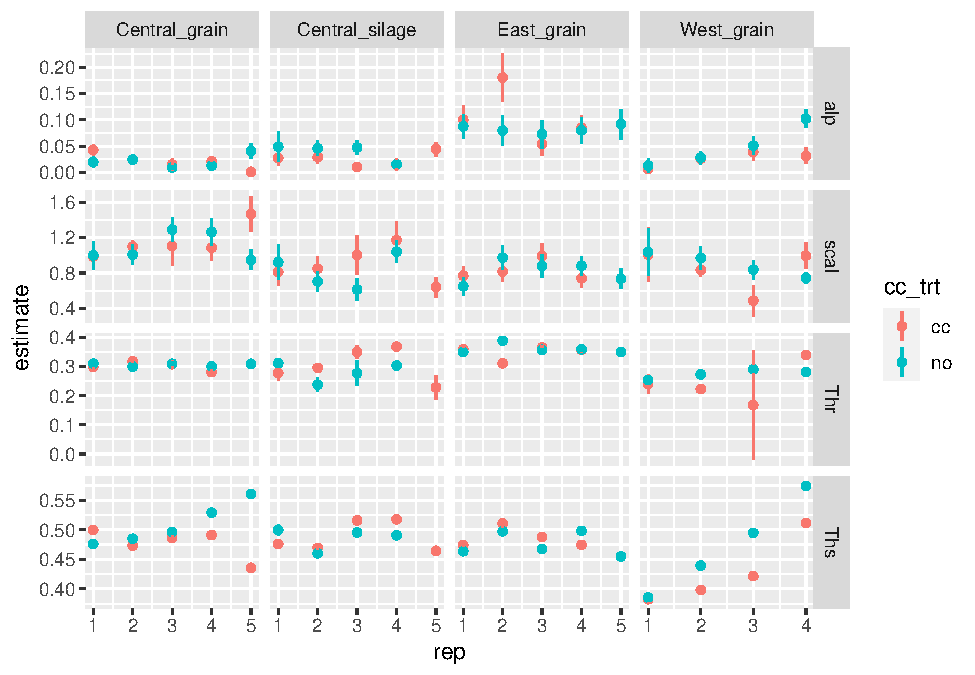
\includegraphics{rmd-supp-mat_files/figure-latex/paramsalp-1.pdf}
\caption{Non-linear model fitted parameters}
\end{figure}

\hypertarget{supplemental-material-s5.-macromicropore-results}{%
\section{Supplemental Material S5. Macro/micropore
results}\label{supplemental-material-s5.-macromicropore-results}}

\begin{figure}
\centering
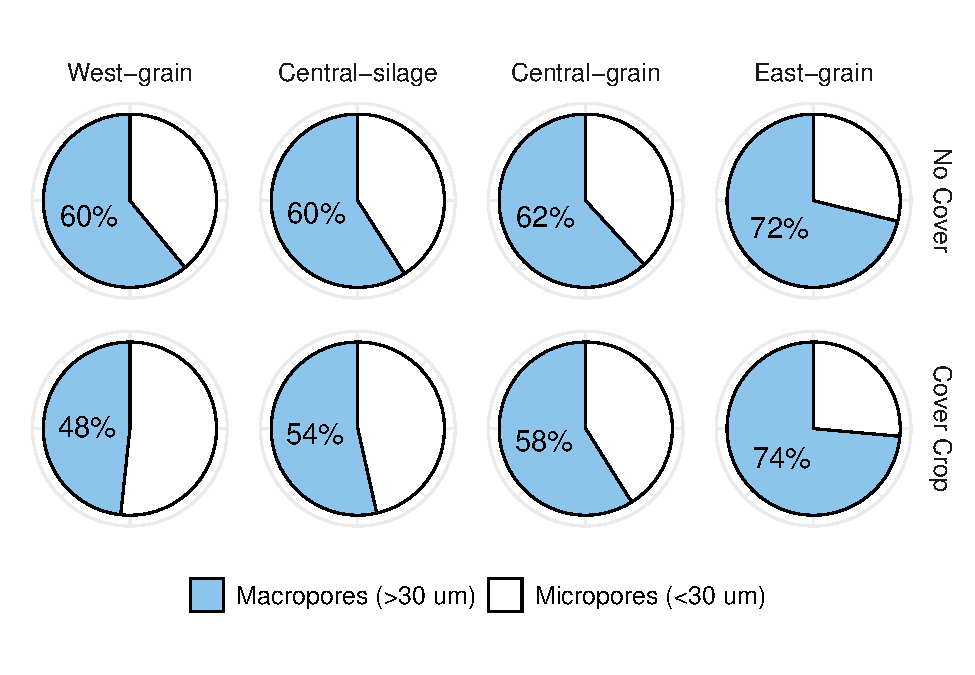
\includegraphics{rmd-supp-mat_files/figure-latex/pores-1.pdf}
\caption{Mean percentage macropores (\textgreater30 µm) for each trial;
percent macropores in the cover crop treatment was significantly lower
(p=0.04) at the West-grain trial compared to the control treatment}
\end{figure}

\end{document}
